%%-----------------------------------------------------------------------%%
%%--- Graph Algorithms --------------------------------------------------%%

\chapter{Graph Algorithms}
\label{chap:graph_algorithms}

Graph algorithms have many applications. Suppose you are a salesman
with a product you would like to sell in several cities. To determine
the cheapest travel route from city-to-city, you must effectively
search a graph having weighted edges for the ``cheapest'' route
visiting each city once. Each vertex denotes a city you must visit and
each edge has a weight indicating either the distance from one city to
another or the cost to travel from one city to another.

Shortest path algorithms are some of the most important algorithms in
algorithmic graph theory. We shall examine several in this chapter.


%%-----------------------------------------------------------------------%%
%%--- Representing graphs in a computer ---------------------------------%%

\section{Representing graphs in a computer}

In section~\ref{sec:introduction:matrix_representation}, we discussed
how to use matrices for representing graphs and digraphs. If
$A = [a_{ij}]$ is an $m \times n$ matrix, the adjacency matrix
representation of a graph would require representing all the $mn$
entries of $A$. Alternative graph representations exist that are much
more efficient than representing all entries of a matrix.


%%--- Adjacency lists ---------------------------------------------------%%

\subsection{Adjacency lists}

A \emph{list} is a sequence of objects. Unlike sets, a list may
contain multiple copies of the same object. Each object of a list is
referred to as an \emph{element} of the list. A list $L$ of
$n \geq 0$ elements is written as $L = [a_1, a_2, \dots, a_n]$, where
the $i$-th element $a_i$ can be indexed as $L[i]$. In case $n = 0$,
the list $L = [\,]$ is referred to as the \emph{empty list}. Two lists
are equivalent if they both contain the same elements at exactly the
same positions.

Define the adjacency lists of a graph as follows. Let $G$ be a graph
with vertex set $V = \{v_1, v_2, \dots, v_n\}$. Assign to each vertex
$v_i$ a list $L_i$ containing all the vertices that are adjacent to
$v_i$. The list $L_i$ associated with $v_i$ is referred to as the
\emph{adjacency list} of $v_i$. Then $L_i = [\,]$ if and only if $v_i$
is an isolated vertex. We say that $L_i$ is \emph{the} adjacency list
of $v_i$ because any permutation of the elements of $L_i$ results in a
list that contains the same vertices adjacent to $v_i$. If each
adjacency list $L_i$ contains $s_i$ elements where
$0 \leq s_i \leq n$, we say that $L_i$ has \emph{length} $s_i$. The
adjacency list representation of the graph $G$ requires that we
represent $\sum_i s_i = 2 \cdot |E(G)| \leq n^2$ elements in a
computer's memory, since each edge appears twice in the adjacency list
representation. An adjacency list is explicit about which vertices are
adjacent to a vertex, and implicit about which vertices are not
adjacent to that same vertex. Without knowing the graph $G$, given the
adjacency lists $L_1, L_2, \dots, L_n$, we can reconstruct $G$. For
example, Figure~\ref{fig:graph_algorithms:graph_adjacency_lists} shows
a graph and its adjacency list representation.

\begin{figure}[!htbp]
\centering
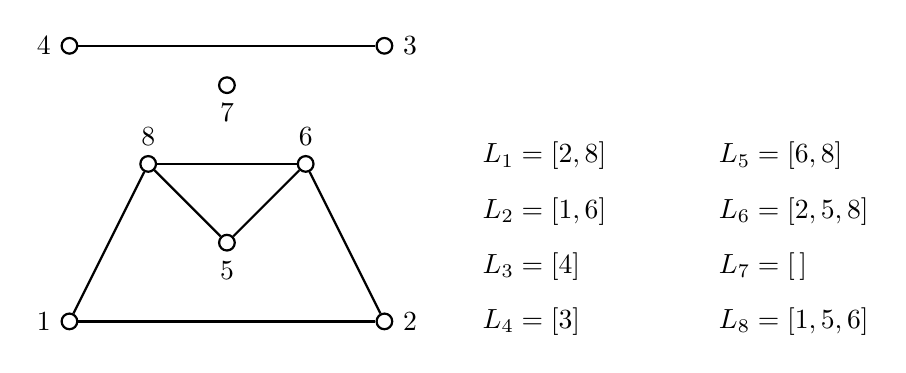
\begin{tikzpicture}
[nodedecorate/.style={shape=circle,inner sep=2pt,draw,thick},%
  linedecorate/.style={-,thick}]
%% nodes or vertices
\foreach \nodename/\x/\y/\direction/\navigate in {
  1/0/0/left/west, 2/4/0/right/east, 3/4/3.5/right/east,
  4/0/3.5/left/west, 5/2/1/below/south, 6/3/2/above/north,
  7/2/3/below/south, 8/1/2/above/north} {
  \node (\nodename) at (\x,\y) [nodedecorate] {};
  \node [\direction] at (\nodename.\navigate) {$\nodename$};
}
%% adjacency lists
\node (L1) at (5,2.1) [] {};
\node [right] at (L1.east) {$L_1 = [2,8]$};
\node (L2) at (5,1.4) [] {};
\node [right] at (L2.east) {$L_2 = [1,6]$};
\node (L3) at (5,0.7) [] {};
\node [right] at (L3.east) {$L_3 = [4]$};
\node (L4) at (5,0) [] {};
\node [right] at (L4.east) {$L_4 = [3]$};
\node (L5) at (8,2.1) [] {};
\node [right] at (L5.east) {$L_5 = [6,8]$};
\node (L6) at (8,1.4) [] {};
\node [right] at (L6.east) {$L_6 = [2,5,8]$};
\node (L7) at (8,0.7) [] {};
\node [right] at (L7.east) {$L_7 = [\,]$};
\node (L8) at (8,0) [] {};
\node [right] at (L8.east) {$L_8 = [1,5,6]$};
%% edges or lines
\path
\foreach \startnode/\endnode in {1/2, 1/8, 2/6, 3/4, 5/6, 5/8, 6/8} {
  (\startnode) edge[linedecorate] node {} (\endnode)
};
\end{tikzpicture}
\caption{A graph and its adjacency lists.}
\label{fig:graph_algorithms:graph_adjacency_lists}
\end{figure}


%%--- The graph6 format -------------------------------------------------%%

\subsection{The graph6 format}

The graph formats graph6 and sparse6 were developed by Brendan
McKay~\cite{McKay2010} at The Australian National University as a
compact way to represent graphs. These two formats use bit vectors and
printable characters of the American Standard Code for Information
Interchange~(ASCII) encoding scheme. The 64 printable ASCII characters
used in graph6 and sparse6 are those ASCII characters with decimal
codes from 63 to 126, inclusive, as shown in
Table~\ref{tab:graph_algorithms:graph6_sparse6_ASCII_printable_characters}.
This section shall only cover the graph6 format. For full
specification on both of the graph6 and sparse6 formats, see
McKay~\cite{McKay2010}.

\begin{table}[!htbp]
\centering
\begin{tabular}{|ccc|ccc|} \hline
binary         & decimal   & glyph    & binary & decimal & glyph \\\hline\hline
\verb!0111111! & \verb!63! & \verb!?! & \verb!1011111! & \verb!95!  & \verb!_! \\
\verb!1000000! & \verb!64! & \verb!@! & \verb!1100000! & \verb!96!  & \verb!`! \\
\verb!1000001! & \verb!65! & \verb!A! & \verb!1100001! & \verb!97!  & \verb!a! \\
\verb!1000010! & \verb!66! & \verb!B! & \verb!1100010! & \verb!98!  & \verb!b! \\
\verb!1000011! & \verb!67! & \verb!C! & \verb!1100011! & \verb!99!  & \verb!c! \\
\verb!1000100! & \verb!68! & \verb!D! & \verb!1100100! & \verb!100! & \verb!d! \\
\verb!1000101! & \verb!69! & \verb!E! & \verb!1100101! & \verb!101! & \verb!e! \\
\verb!1000110! & \verb!70! & \verb!F! & \verb!1100110! & \verb!102! & \verb!f! \\
\verb!1000111! & \verb!71! & \verb!G! & \verb!1100111! & \verb!103! & \verb!g! \\
\verb!1001000! & \verb!72! & \verb!H! & \verb!1101000! & \verb!104! & \verb!h! \\
\verb!1001001! & \verb!73! & \verb!I! & \verb!1101001! & \verb!105! & \verb!i! \\
\verb!1001010! & \verb!74! & \verb!J! & \verb!1101010! & \verb!106! & \verb!j! \\
\verb!1001011! & \verb!75! & \verb!K! & \verb!1101011! & \verb!107! & \verb!k! \\
\verb!1001100! & \verb!76! & \verb!L! & \verb!1101100! & \verb!108! & \verb!l! \\
\verb!1001101! & \verb!77! & \verb!M! & \verb!1101101! & \verb!109! & \verb!m! \\
\verb!1001110! & \verb!78! & \verb!N! & \verb!1101110! & \verb!110! & \verb!n! \\
\verb!1001111! & \verb!79! & \verb!O! & \verb!1101111! & \verb!111! & \verb!o! \\
\verb!1010000! & \verb!80! & \verb!P! & \verb!1110000! & \verb!112! & \verb!p! \\
\verb!1010001! & \verb!81! & \verb!Q! & \verb!1110001! & \verb!113! & \verb!q! \\
\verb!1010010! & \verb!82! & \verb!R! & \verb!1110010! & \verb!114! & \verb!r! \\
\verb!1010011! & \verb!83! & \verb!S! & \verb!1110011! & \verb!115! & \verb!s! \\
\verb!1010100! & \verb!84! & \verb!T! & \verb!1110100! & \verb!116! & \verb!t! \\
\verb!1010101! & \verb!85! & \verb!U! & \verb!1110101! & \verb!117! & \verb!u! \\
\verb!1010110! & \verb!86! & \verb!V! & \verb!1110110! & \verb!118! & \verb!v! \\
\verb!1010111! & \verb!87! & \verb!W! & \verb!1110111! & \verb!119! & \verb!w! \\
\verb!1011000! & \verb!88! & \verb!X! & \verb!1111000! & \verb!120! & \verb!x! \\
\verb!1011001! & \verb!89! & \verb!Y! & \verb!1111001! & \verb!121! & \verb!y! \\
\verb!1011010! & \verb!90! & \verb!Z! & \verb!1111010! & \verb!122! & \verb!z! \\
\verb!1011011! & \verb!91! & \verb![! & \verb!1111011! & \verb!123! & \verb!{! \\
\verb!1011100! & \verb!92! & \verb!\! & \verb!1111100! & \verb!124! & \verb!|! \\
\verb!1011101! & \verb!93! & \verb!]! & \verb!1111101! & \verb!125! & \verb!}! \\
\verb!1011110! & \verb!94! & \verb!^! & \verb!1111110! & \verb!126! & \verb!~! \\\hline
\end{tabular}
\caption{ASCII printable characters used by graph6 and sparse6.}
\label{tab:graph_algorithms:graph6_sparse6_ASCII_printable_characters}
\end{table}


%%--- Bit vectors -------------------------------------------------------%%

\subsubsection{Bit vectors}

Before discussing how graph6 and sparse6 represent graphs using
printable ASCII characters, we first present encoding schemes used by
these two formats. A \emph{bit vector} is, as its name suggests, a
vector whose elements are 1's and 0's. It can be represented as a list
of bits, e.g. \verb!E! can be represented as the ASCII bit vector
$[\texttt{1}, \texttt{0}, \texttt{0}, \texttt{0}, \texttt{1},
  \texttt{0}, \texttt{1}]$. For brevity, we write a bit vector in a
compact form such as \texttt{1000101}. The \emph{length} of a bit
vector is its number of bits. The \emph{most significant bit}
of a bit vector $v$ is the bit position with the largest value among
all the bit positions in $v$. Similarly, the
\emph{least significant bit} is the bit position in $v$ having the
least value among all the bit positions in $v$. The least significant
bit of $v$ is usually called the parity bit because when $v$
interpreted as an integer the parity bit determines whether the
integer is even or odd. Reading \texttt{1000101} from left to right,
the first bit \texttt{1} is the most significant bit, followed by the
second bit \texttt{0} which is the second most significant bit, and so
on all the way down to the seventh bit \texttt{1} which is the least
significant bit.

The order in which we process the bits of a bit vector is referred to
as \emph{endianness}. Processing $v$ in \emph{big-endian} order means
that we first process the most significant bit of $v$, followed by the
second most significant bit, and so on all the way down to the least
significant bit of $v$. \emph{Little-endian} order means that we first
process the least significant bit, followed by the second least
significant bit, and so on all the way up to the most significant
bit. In big-endian order, the ASCII binary representation of
\texttt{E} is written \texttt{1000101}~(see
Table~\ref{tab:graph_algorithms:big_endian_ASCII_binary_E}), while
the little-ending order is written \texttt{1010001}~(see
Table~\ref{tab:graph_algorithms:little_endian_ASCII_binary_E}). To
determine the integer representation of a bit vector, multiply each
bit value by its corresponding position value, then add up all the
results. In general, if the bit vector $v = b_1 b_2 \cdots b_k$ is the
big-endian binary representation of a positive integer, then the
integer representation of $v$ is
%
\begin{equation}
\label{eq:graph_algorithms:big_endian_binary_to_integer}
\sum_{i=1}^k 2^{k-i} b_i
=
2^{k-1} b_1 + 2^{k-2} b_2 + 2^{k-3} b_3 + \cdots + 2^0 b_k.
\end{equation}

\begin{table}[!htbp]
\centering
\begin{tabular}{|l|ccccccc|} \hline
position       & 1          & 2          & 3          & 4          & 5          & 6          & 7 \\\hline
bit value      & \texttt{1} & \texttt{0} & \texttt{0} & \texttt{0} & \texttt{1} & \texttt{0} & \texttt{1} \\\hline
position value & $2^6$      & $2^5$      & $2^4$      & $2^3$      & $2^2$      & $2^1$      & $2^0$ \\\hline
\end{tabular}
\caption{Big-endian order of the ASCII binary code of \texttt{E}.}
\label{tab:graph_algorithms:big_endian_ASCII_binary_E}
\end{table}

\begin{table}[!htbp]
\centering
\begin{tabular}{|l|ccccccc|} \hline
position       & 1          & 2          & 3          & 4          & 5          & 6          & 7 \\\hline
bit value      & \texttt{1} & \texttt{0} & \texttt{1} & \texttt{0} & \texttt{0} & \texttt{0} & \texttt{1} \\\hline
position value & $2^0$      & $2^1$      & $2^2$      & $2^3$      & $2^4$      & $2^5$      & $2^6$ \\\hline
\end{tabular}
\caption{Little-endian order of the ASCII binary code of \texttt{E}.}
\label{tab:graph_algorithms:little_endian_ASCII_binary_E}
\end{table}

In graph6 and sparse6 formats, the length of a bit vector must be a
multiple of 6. Suppose $v$ is a bit vector of length $k$ such that
$6 \nmid k$. To transform $v$ into a bit vector having length a
multiple of 6, let $r = k \mod 6$ be the remainder upon dividing $k$
by 6, and pad $6 - r$ zeros to the right of $v$.

Suppose $v = b_1 b_2 \cdots b_k$ is a bit vector of length $k$, where
$6 \;|\; k$. We split $v$ into $k/6$ bit vectors $v_i$, each of length
6. For $0 \leq i \leq k/6$, the $i$-th bit vector is given by
\[
v_i
=
b_{6i-5} b_{6i-4} b_{6i-3} b_{6i-2} b_{6i-1} b_{6i}.
\]
Consider each $v_i$ as the big-endian binary representation of a
positive
integer. Use~(\ref{eq:graph_algorithms:big_endian_binary_to_integer})
to obtain the integer representation $N_i$ of each $v_i$. Then add 63
to each $N_i$ to obtain $N_i'$ and store $N_i'$ in one byte of
memory. That is, each $N_i'$ can be represented as a bit vector of
length $8$. Thus the required number of bytes to store $v$ is
$\lceil k/6 \rceil$. Let $B_i$ be the byte representation of $N_i'$ so
that
%
\begin{equation}
\label{eq:graph_algorithms:byte_representation_bit_vector}
R(v)
=
B_1 B_2 \cdots B_{\lceil k/6 \rceil}
\end{equation}
%
denotes the representation of $v$ as a sequence of $\lceil k/6 \rceil$
bytes.

We now discuss how to encode an integer $n$ in the range
$0 \leq n \leq 2^{36} - 1$
using~(\ref{eq:graph_algorithms:byte_representation_bit_vector}) and
denote such an encoding of $n$ as $N(n)$. Let $v$ be the big-endian
binary representation of $n$. Then $N(n)$ is given by
%
\begin{equation}
\label{eq:graph_algorithms:graph6_sparse6_graph_orders}
N(n)
=
\begin{cases}
n + 63, & \text{if $0 \leq n \leq 62$}, \\
126 \, R(v), & \text{if $63 \leq n \leq 258047$}, \\
126 \, 126 \, R(v), & \text{if $258048 \leq n \leq 2^{36}-1$}.
\end{cases}
\end{equation}
%% If $0 \leq n \leq 62$, then
%% we write $N(n) = n + 63$. If $63 \leq n \leq 258047$, let $v$ be the
%% big-endian binary representation of $n$ and write
%% $N(n) = 126 \, R(v)$. Finally, if $258048 \leq n \leq 2^{36} - 1$,
%% again we let $v$ be the big-endian binary representation of $n$ and
%% write $N(n) = 126 \, 126 \, R(v)$.
Note that $n + 63$ requires one byte of storage memory, while
$126 \, R(v)$ and $126 \, 126 \, R(v)$ require 4 and 8 bytes,
respectively.


%%--- The graph6 format -------------------------------------------------%%

\subsubsection{The graph6 format}

The graph6 format is used to represent simple, undirected graphs of
order from $0$ to $2^{36} - 1$, inclusive. Let $G$ be a simple,
undirected graph of order $0 \leq n \leq 2^{36} - 1$. If $n = 0$, then
$G$ is represented in graph6 format as ``\verb!?!''. Suppose $n >
0$. Let $M = [a_{ij}]$ be the adjacency matrix of $G$. Consider the
upper triangle of $M$, excluding the main diagonal, and write that
upper triangle as the bit vector
\[
v
=
\underbrace{a_{0,1}}_{c_1}
\underbrace{a_{0,2} a_{1,2}}_{c_2}
\underbrace{a_{0,3} a_{1,3} a_{2,3}}_{c_3} \cdots
\underbrace{a_{0,i} a_{1,i} \cdots a_{i-1,i}}_{c_i} \cdots
\underbrace{a_{0,n} a_{1,n} \cdots a_{n-1,n}}_{c_n}
\]
where $c_i$ denotes the entries $a_{0,i} a_{1,i} \cdots a_{i-1,i}$ in
column $i$ of $M$. Then the graph6 representation of $G$ is
$N(n) R(v)$, where $R(v)$ and $N(n)$ are as
in~(\ref{eq:graph_algorithms:byte_representation_bit_vector})
and~(\ref{eq:graph_algorithms:graph6_sparse6_graph_orders}),
respectively. That is, $N(n)$ encodes the order of $G$ and $R(v)$
encodes the edges of $G$.


%%-----------------------------------------------------------------------%%
%%--- Graph searching ---------------------------------------------------%%

\section{Graph searching}
\label{sec:graph_algorithms:graph_searching}

%% This section discusses algorithms for
%%
%% \begin{itemize}
%% \item
%% breadth-first searches,
%%
%% \item
%% depth-first searches, and
%%
%% \item
%% we explain how these relate to determining a graph's connectivity.
%% \end{itemize}

This section discusses two fundamental algorithms for graph traversal:
breadth-first search and depth-first search. The word ``search'' used
in describing these two algorithms is rather misleading. It would be
more accurate to describe them as algorithms for constructing trees
using the adjacency information of a given graph. However, the names
``breadth-first search'' and ``depth-first search'' are entrenched in
literature on graph theory and computer science. From hereon, we use
these two names as given above, bearing in mind their intended
purposes.


%%--- Breadth-first search ----------------------------------------------%%

\subsection{Breadth-first search}

Breadth-first search (BFS) is a strategy for running through the
vertices of a graph. It was presented by Moore~\cite{Moore1959} in
1959 within the context of traversing mazes. Lee~\cite{Lee1961}
independently discovered the same algorithm in 1961 in his work on
routing wires on circuit boards.

The basic BFS algorithm can be described as follows. Starting from a
given vertex $v$ of a graph $G$, we first explore the neighborhood of
$v$ by visiting all vertices that are adjacent to $v$. We then apply
the same strategy to each of the neighbors of $v$. The strategy of
exploring the neighborhood of a vertex is applied to all vertices of
$G$. The result is a tree rooted at $v$ and this tree is a subgraph of
$G$. Algorithm~\ref{alg:graph_algorithms:breadth_first_search_template}
presents a general template for the BFS strategy. The tree resulting
from the BFS algorithm is called a \emph{breadth-first search tree}.
\index{BFS}
\index{breadth-first search}

\begin{algorithm}[!htpb]
\dontprintsemicolon  % no semicolon at end of pseudocode statements
%% data section
\SetKwInOut{Input}{Input}
\SetKwInOut{Output}{Output}
%% input/output
\Input{A directed or undirected graph $G = (V, E)$ of order $n > 0$. A
  vertex $s$ from which to start the search. The vertices are numbered
  from $1$ to  $n = |V|$, i.e. $V = \{1, 2, \dots, n\}$.}
\Output{A list $D$ of distances of all vertices from $s$. A tree $T$
  rooted at $s$.}
\BlankLine
$Q \leftarrow [s]$~\nllabel{alg:BFS:initialize_queue_visit_nodes} \tcc*[f]{queue of nodes to visit}\;
$D \leftarrow [\infty, \infty, \dots, \infty]$ \tcc*[f]{$n$ copies of $\infty$}\;
$D[s] \leftarrow 0$\;
$T \leftarrow [\,]$~\nllabel{alg:BFS:initialize_empty_tree}\;
\While{$\length(Q) > 0$~\nllabel{alg:BFS:while_loop:non_empty_queue}}{
  $v \leftarrow \dequeue(Q)$\;
  \For{\emph{each} $w \in \adj(v)$~\nllabel{alg:BFS:explore_neighborhood}}{
    \If{$D[w] = \infty$~\nllabel{alg:BFS:marking_vertex_as_visited}}{
      $D[w] \leftarrow D[v] + 1$\;
      $\enqueue(Q, w)$\;
      $\append(T, vw)$~\nllabel{alg:BFS:while_loop:append_to_tree}\;
    }
  }
}
\Return $(D, T)$\;
\caption{A general breadth-first search template.}
\label{alg:graph_algorithms:breadth_first_search_template}
\end{algorithm}

The breadth-first search algorithm makes use of a special type of list
called a \emph{queue}. This is analogous to a queue of people waiting
in line to be served. A person may enter the queue by joining the rear
of the queue. The person who is in the queue the longest amount of
time is served first, followed by the person who has waited the second
longest time, and so on. Formally, a queue $Q$ is a list of
elements. At any time, we only have access to the first element of
$Q$, known as the \emph{front} or \emph{start} of the queue. We insert
a new element into $Q$ by appending the new element to the \emph{rear}
or \emph{end} of the queue. The operation of removing the front of $Q$
is referred to as \emph{dequeue}, while the operation of appending to
the rear of $Q$ is called \emph{enqueue}. That is, a queue implements
a first-in first-out~(FIFO) protocol for adding and moving
elements. As with lists, the \emph{length} of a queue is its total
number of elements.

\begin{figure}[!htbp]
\centering
\subfigure[]{
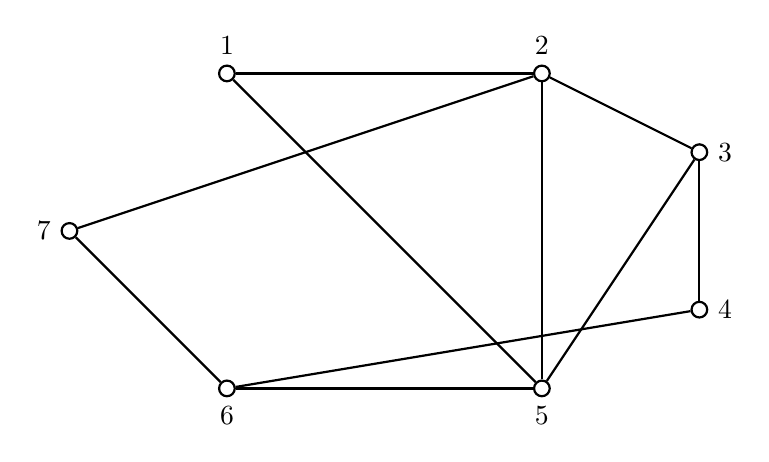
\begin{tikzpicture}
[nodedecorate/.style={shape=circle,inner sep=2pt,draw,thick},%
  linedecorate/.style={-,thick}]
%% nodes or vertices
\foreach \nodename/\x/\y/\direction/\navigate in {2/4/4/above/north,
  1/0/4/above/north, 3/6/3/right/east, 4/6/1/right/east,
  5/4/0/below/south, 7/-2/2/left/west, 6/0/0/below/south} {
  \node (\nodename) at (\x,\y) [nodedecorate] {};
  \node [\direction] at (\nodename.\navigate) {$\nodename$};
}
%% edges or lines
\path
\foreach \startnode/\endnode in {1/2, 1/5, 2/3, 2/5, 2/7, 3/4, 3/5,
  4/6, 5/6, 6/7} {
  (\startnode) edge[linedecorate] node {} (\endnode)
};
\end{tikzpicture}
}
%%
\qquad
\subfigure[]{
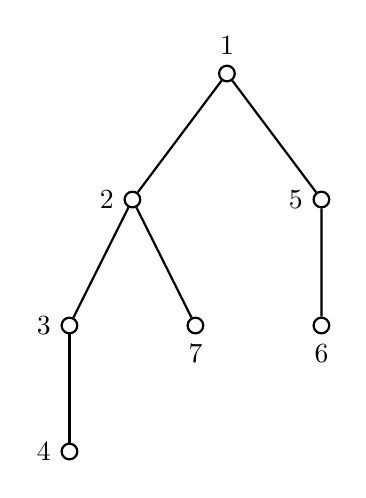
\begin{tikzpicture}
[nodedecorate/.style={shape=circle,inner sep=2pt,draw,thick},%
  linedecorate/.style={-,thick},%
  scale=1.6]
%% nodes or vertices
\foreach \nodename/\x/\y/\direction/\navigate in {4/0/0/left/west,
  3/0/1/left/west, 7/1/1/below/south, 6/2/1/below/south,
  2/0.5/2/left/west, 5/2/2/left/west, 1/1.25/3/above/north} {
  \node (\nodename) at (\x,\y) [nodedecorate] {};
  \node [\direction] at (\nodename.\navigate) {$\nodename$};
}
%% edges or lines
\path
\foreach \startnode/\endnode in {1/2, 1/5, 2/3, 2/7, 3/4, 5/6} {
  (\startnode) edge[linedecorate] node {} (\endnode)
};
\end{tikzpicture}
}
%%
%%
\subfigure[]{
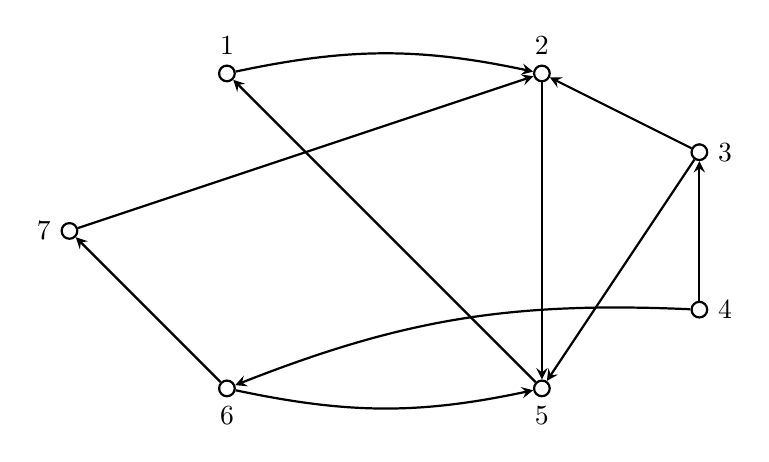
\begin{tikzpicture}
[nodedecorate/.style={shape=circle,inner sep=2pt,draw,thick},%
  arrowdecorate/.style={->,>=stealth,thick}]
%% nodes or vertices
\foreach \nodename/\x/\y/\direction/\navigate in {2/4/4/above/north,
  1/0/4/above/north, 3/6/3/right/east, 4/6/1/right/east,
  5/4/0/below/south, 7/-2/2/left/west, 6/0/0/below/south} {
  \node (\nodename) at (\x,\y) [nodedecorate] {};
  \node [\direction] at (\nodename.\navigate) {$\nodename$};
}
%% edges or lines
\path
\foreach \startnode/\endnode in {2/5, 3/2, 3/5, 4/3, 5/1, 6/7, 7/2} {
  (\startnode) edge[arrowdecorate] node {} (\endnode)
}
\foreach \startnode/\endnode/\benddirection/\angle in {
  1/2/bend left/12, 4/6/bend right/12, 6/5/bend right/12} {
  (\startnode) edge[arrowdecorate,\benddirection=\angle] node {} (\endnode)
};
\end{tikzpicture}
}
%%
\qquad
\subfigure[]{
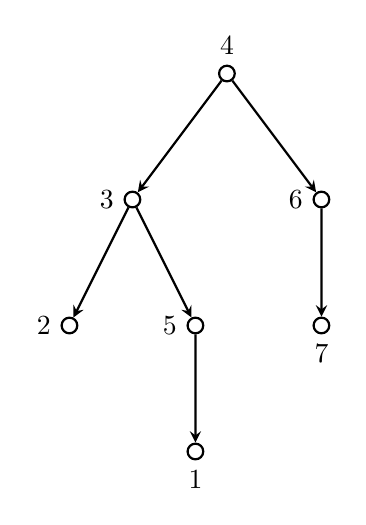
\begin{tikzpicture}
[nodedecorate/.style={shape=circle,inner sep=2pt,draw,thick},%
  arrowdecorate/.style={->,>=stealth,thick},
  scale=1.6]
%% nodes or vertices
\foreach \nodename/\x/\y/\direction/\navigate in {2/0/1/left/west,
  1/1/0/below/south, 5/1/1/left/west, 7/2/1/below/south,
  6/2/2/left/west, 3/0.5/2/left/west, 4/1.25/3/above/north} {
  \node (\nodename) at (\x,\y) [nodedecorate] {};
  \node [\direction] at (\nodename.\navigate) {$\nodename$};
}
%% edges or lines
\path
\foreach \startnode/\endnode in {4/3, 4/6, 3/2, 3/5, 6/7, 5/1} {
  (\startnode) edge[arrowdecorate] node {} (\endnode)
};
\end{tikzpicture}
}
\caption{Breadth-first search trees for undirected and directed graphs.}
\label{fig:graph_algorithms:bread_first_search_undirected}
\end{figure}

Note that the BFS
Algorithm~\ref{alg:graph_algorithms:breadth_first_search_template}
works on both undirected and directed graphs. For an undirected graph,
line~\ref{alg:BFS:explore_neighborhood} means that we explore all
the neighbors of vertex $v$, i.e. the set $\adj(v)$ of vertices
adjacent to $v$. In the case of a digraph, we replace $w \in \adj(v)$
in line~\ref{alg:BFS:explore_neighborhood} with $w \in \oadj(v)$
because we only want to explore all vertices that are out-neighbors of
$v$. The algorithm returns two lists $D$ and $T$. The list $T$
contains a subset of edges in $E(G)$ that make up a tree rooted at the
given start vertex $s$. As trees are connected graphs without cycles,
we may take the vertices comprising the edges of $T$ to be the vertex
set of the tree. The list $D$ has the same number of elements as the
order of $G = (V, E)$, i.e. $\length(D) = |V|$. The $i$-th element
$D[i]$ counts the number of edges in $T$ between the vertices $s$ and
$v_i$. In other words, $D[i]$ is the length of the $s$-$v_i$ path. It
can be shown that $D[i] = \infty$ if and only if $G$ is
disconnected. After one application of
Algorithm~\ref{alg:graph_algorithms:breadth_first_search_template}, it
may happen that $D[i] = \infty$ for at least one vertex
$v_i \in V$. To traverse those vertices that are unreachable from $s$,
again we apply
Algorithm~\ref{alg:graph_algorithms:breadth_first_search_template} on
$G$ with starting vertex $v_i$. Repeat this algorithm as often as
necessary until all vertices of $G$ are visited. The result may be a
tree that contains all the vertices of $G$ or a collection of trees,
each of which contains a subset of $V(G)$.
Figure~\ref{fig:graph_algorithms:bread_first_search_undirected}
presents BFS trees resulting from applying
Algorithm~\ref{alg:graph_algorithms:breadth_first_search_template} on
an undirected graph and a digraph.

\begin{theorem}
The worst-case time complexity of
Algorithm~\ref{alg:graph_algorithms:breadth_first_search_template} is
$O(|V| + |E|)$.
\end{theorem}

\begin{proof}
Without loss of generality, we can assume that $G = (V, E)$ is
connected. The initialization steps in
lines~\ref{alg:BFS:initialize_queue_visit_nodes}
to~\ref{alg:BFS:initialize_empty_tree} take $O(|V|)$ time. After
initialization, all but one vertex are labelled
$\infty$. Line~\ref{alg:BFS:marking_vertex_as_visited} ensures that
each vertex is enqueued at most once and hence dequeued at most
once. Each of enqueuing and dequeuing takes constant time. The total
time devoted to queue operations is $O(|V|)$. The adjacency list of a
vertex is scanned after dequeuing that vertex, so each adjacency list
is scanned at most once. Summing the lengths of the adjacency lists,
we have $\Theta(|E|)$ and therefore we require $O(|E|)$ time to scan
the adjacency lists. After the adjacency list of a vertex is scanned,
at most $k$ edges are added to the list $T$, where $k$ is the length
of the adjacency list under consideration. Like queue operations,
appending to a list takes constant time, hence we require $O(|E|)$
time to build the list $T$. Therefore, BFS runs in $O(|V| + |E|)$
time.
\end{proof}

\begin{theorem}
For the list $D$ resulting from
Algorithm~\ref{alg:graph_algorithms:breadth_first_search_template},
let $s$ be a starting vertex and let $v$ be a vertex such that
$D[v] \neq \infty$. Then $D[v]$ is the length of any shortest path
from $s$ to $v$.
\end{theorem}

\begin{proof}
It is clear that $D[v] = \infty$ if and only if there are no paths
from $s$ to $v$. Let $v$ be a vertex such that $D[v] \neq \infty$. As
$v$ can be reached from $s$ by a path of length $D[v]$, the length
$d(s,v)$ of any shortest $s$-$v$ path satisfies $d(s,v) \leq
D[v]$. Use induction on $d(s,v)$ to show that equality holds. For the
base case $s = v$, we have $d(s,v) = D[v] = 0$ since the trivial path
has length zero. Assume for induction that if $d(s,v) = k$, then
$d(s,v) = D[v]$.
%% We need to show that if $d(s,u)$ is the length of any
%% shortest $s$-$u$ path, then $d(s,u) = D[u]$.
Let $d(s,u) = k + 1$ with the corresponding shortest $s$-$u$ path
being $(s, v_1, v_2, \dots, v_k, u)$. Then by our induction
hypothesis, $(s, v_1, v_2, \dots, v_k)$ is a shortest path from $s$ to
$v_k$ of length $d(s, v_k) = D[v_k] = k$. In other words, $D[v_k] <
D[u]$ and the while loop spanning
lines~\ref{alg:BFS:while_loop:non_empty_queue}
to~\ref{alg:BFS:while_loop:append_to_tree} processes $v_k$ before
processing $u$. The graph under consideration has the edge $v_k
u$. When examining the adjacency list of $v_k$, BFS reaches $u$~(if
$u$ is not reached earlier) and so $D[u] \leq k + 1$. Hence,
$D[u] = k + 1$ and therefore $d(s,u) = D[u] = k + 1$.
\end{proof}

%% Another version of
%% Algorithm~\ref{alg:graph_algorithms:breadth_first_search} is where you
%% are searching the graph for a vertex (or edge) satisfying a certain
%% property $P$. In that situation, you simply quit at the step where you
%% increment the counter, i.e. line~7 in
%% Algorithm~\ref{alg:graph_algorithms:breadth_first_search}. Other
%% variations are also possible as well.

%% For the example of the graph in
%% Figure~\ref{fig:introduction:types_of_walks}, the list of distances
%% from vertex \verb!a! to any other vertex is
%% %
%% \begin{center}
%% \fontsize{9pt}{9pt}
%% \selectfont
%% \tt
%% \begin{lstlisting}
%% [['a', 0], ['b', 1], ['c', 2], ['d', 3], ['e', 1], ['f', 2], ['g', 2]]
%% \end{lstlisting}
%% \end{center}
%% %
%% To create this list,
%% %
%% \begin{itemize}
%% \item
%% Start at \verb!a! and compute the distance from \verb!a! to itself.

%% \item
%% Move to each neighbor of \verb!a!, namely \verb!b! and \verb!e!, and
%% compute the distance from \verb!a! to each of them.

%% \item
%% Move to each ``unseen'' neighbor of \verb!b!, namely just \verb!c!,
%% and compute the distance from \verb!a! to it.

%% \item
%% Move to each ``unseen'' neighbor of \verb!e!, namely just \verb!f!,
%% and compute the distance from \verb!a! to it.

%% \item
%% Move to each ``unseen'' neighbor of \verb!c!, namely just \verb!d!,
%% and compute the distance from \verb!a! to it.

%% \item
%% Move to each ``unseen'' neighbor of \verb!f!, namely just \verb!g!,
%% and compute the distance from \verb!a! to it.
%% \end{itemize}

%% As an example, here is some Sage code which implements BFS to compute
%% the list distances from a given vertex.
%% %
%% \begin{center}
%% \fontsize{9pt}{9pt}
%% \selectfont
%% \tt
%% \begin{lstlisting}
%% def graph_distance(G, v0):
%%     """
%%     Breadth first search algorithm to find the
%%     distance from a fixed vertex $v_0$ to any
%%     other vertex.

%%     INPUT:
%%         G - a connected graph
%%         v0 - a vertex

%%     OUTPUT:
%%         D - a list of distances to
%%             every other vertex

%%     EXAMPLES:
%%         sage: G = Graph({1: [2, 4], 2: [1, 4], 3: [2, 6],
%%                          4: [1, 3], 5: [4, 2], 6: [3, 1]})
%%         sage: v0 = 1
%%         sage: graph_distance(G,v0)
%%         [[1, 0], [2, 1], [3, 2], [4, 1], [5, 2], [6, 1]]
%%         sage: G = Graph({"a": ["b", "e"], "b": ["c", "e"], \
%%          "c": ["d", "e"], "d": ["f"], "e": ["f"], "f": ["g"], "g":["b"]})
%%         sage: v0 = "a"
%%         sage: graph_distance(G, v0)
%%         [['a', 0], ['b', 1], ['c', 2], ['d', 3], ['e', 1],
%%          ['f', 2], ['g', 2]]
%%         sage: G = Graph({1: [2,3], 2: [1, 3], 3: [2], 4: [5], 5: [6], 6: [5]})
%%         sage: v0 = 1
%%         sage: graph_distance(G, v0) # note G is disconnected
%%         [[1, 0], [2, 1], [3, 1]]
%%     """
%%     V = G.vertices()
%%     Q = [v0]
%%     T = []
%%     D = []
%%     while Q<>[] and T<>V:
%%         for v in Q:
%%             if not(v in T):
%%                 D.append([v,G.distance(v0,v)])
%%             if v in Q:
%%                 Q.remove(v)
%%             T.append(v)
%%             T = list(Set(T))
%%             Q = Q+[x for x in G.neighbors(v) if not(x in T+Q)]
%%             if T == V:
%%                 break
%%     D.sort()
%%     print Q, T
%%     return D
%% \end{lstlisting}
%% \end{center}
%% %
%% \begin{exercise}
%% Using Sage's \verb!shortest_path! method, can you modify the above
%% function to return a list of shortest paths from $v_0$ to any other
%% vertex?
%% \end{exercise}


%%--- Depth-first search ------------------------------------------------%%

\subsection{Depth-first search}

A depth-first search~(DFS) is a graph traversal strategy similar to
breadth-first search. Both BFS and DFS differ in how they explore each
vertex. Whereas BFS explores the neighborhood of a vertex $v$ before
moving on to explore the neighborhoods of the neighbors, DFS explores
as deep as possible a path starting at $v$. One can think of BFS as
exploring the immediate surrounding, while DFS prefers to see what is
on the other side of the hill. In the 19th century,
Lucas~\cite{Lucas1882.1894} and Tarry~\cite{Tarry1895} investigated
DFS as a strategy for traversing mazes. Fundamental properties of DFS
were discovered in the early 1970s by Hopcroft and
Tarjan~\cite{HopcroftTarjan1973,Tarjan1972}.

To get an intuitive appreciation for DFS, suppose we have an
$8 \times 8$ chessboard in front of us. We place a single knight
piece on a fixed square of the board. Our objective is to find a
sequence of knight moves that visits each and every square exactly
once, while obeying the rules of chess that govern the movement of the
knight piece. Such a sequence of moves, if one exists, is called a
\emph{knight's tour}. How do we find such a tour? We could make one
knight move after another, recording each move to ensure that we do
not step on a square that is already visited, until we could not make
any more moves. Acknowledging defeat when encountering a dead end, it
might make sense to \emph{backtrack} a few moves and try again, hoping
we would not get stuck. If we fail again, we try backtracking a few
more moves and traverse yet another path, hoping to make further
progress. Repeat this strategy until a tour is found or until we have
exhausted all possible moves. The above strategy for finding a
knight's tour is an example of depth-first search, sometimes called
\emph{backtracking}.
\index{backtracking}
\index{knight's tour}

\begin{algorithm}[!htpb]
\dontprintsemicolon  % no semicolon at end of pseudocode statements
%% data section
\SetKwInOut{Input}{Input}
\SetKwInOut{Output}{Output}
%% input/output
\Input{A directed or undirected graph $G = (V, E)$ of order $n > 0$. A
  vertex $s$ from which to start the search. The vertices are numbered
  from $1$ to  $n = |V|$, i.e. $V = \{1, 2, \dots, n\}$.}
\Output{A list $D$ of distances of all vertices from $s$. A tree $T$
  rooted at $s$.}
\BlankLine
$S \leftarrow [s]$ \tcc*[f]{stack of nodes to visit}\;
$D \leftarrow [\infty, \infty, \dots, \infty]$ \tcc*[f]{$n$ copies of $\infty$}\;
$D[s] \leftarrow 0$\;
$T \leftarrow [\,]$\;
\While{$\length(S) > 0$}{
  $v \leftarrow \pop(S)$\;
  \For{\emph{each} $w \in \adj(v)$}{
    \If{$D[w] = \infty$}{
      $D[w] \leftarrow D[v] + 1$\;
      $\push(S, w)$\;
      $\append(T, vw)$\;
    }
  }
}
\Return $(D, T)$\;
\caption{A general depth-first search template.}
\label{alg:graph_algorithms:depth_first_search_template}
\end{algorithm}

Algorithm~\ref{alg:graph_algorithms:depth_first_search_template}
formalizes the above description of depth-first search. The tree
resulting from applying DFS on a graph is called a
\emph{depth-first search tree}. The general structure of this
algorithm bears close resemblance to
Algorithm~\ref{alg:graph_algorithms:breadth_first_search_template}. A
significant difference is that instead of using a queue to structure
and organize vertices to be visited, DFS uses another special type of
list called a \emph{stack}. To understand how elements of a stack are
organized, we use the analogy of a stack of cards. A new card is added
to the stack by placing it on top of the stack. Any time we want to
remove a card, we are only allowed to remove the top-most card that is
on the top of the stack. A list $L = [a_1, a_2, \dots, a_k]$ of $k$
elements is a stack when we impose the same rules for element
insertion and removal. The top and bottom of the stack are $L[k]$ and
$L[1]$, respectively. The operation of removing the top element of the
stack is referred to as \emph{popping} the element off the
stack. Inserting an element into the stack is called \emph{pushing}
the element onto the stack. In other words, a stack implements a
last-in first-out~(LIFO) protocol for element insertion and removal,
in contrast to the FIFO policy of a queue. We also use the term
\emph{length} to refer to the number of elements in the stack.


%%--- Application: connectivity of a graph ------------------------------%%

\subsection{Application: connectivity of a graph}

% This subsection is on how the above algorithms can be used
% to determine a graph's connectivity.

A simple algorithm to determine if a graph is connected
might be described as follows:
\begin{itemize}

\item
Begin at any arbitrary vertex of the graph, $\Gamma=(V,E)$.

\item
Proceed from that vertex using either DFS or BFS, counting all
vertices reached.

\item
Once the connected component of the graph has been entirely traversed,
if the number of vertices counted is equal to $|V|$,
the graph is connected and otherwise it is disconnected.
\end{itemize}


%%--- Problems ----------------------------------------------------------%%

\subsection*{Problems~\ref{sec:graph_algorithms:graph_searching}}

\begin{enumerate}
\item Let $G = (V, E)$ be an undirected graph, let $s \in V$, and $D$
  is the list of distances resulting from running
  Algorithm~\ref{alg:graph_algorithms:breadth_first_search_template}
  with $G$ and $s$ as input. Show that $G$ is connected if and only if
  $D[v]$ is defined for each $v \in V$.
\end{enumerate}


%%-----------------------------------------------------------------------%%
%%--- Dijkstra's algorithm ----------------------------------------------%%

\section{Shortest path algorithms}


Let $G = (V,E)$ be a graph with non-negative edge weights, $w(e)$ for
$e \in E$. The \emph{length of a path} $P$ from $v \in V$ to $w \in V$ is the sum of
the edge weights for each edge in the path $P$, denoted
$\delta(P)$. We write $\delta(v,w)$ for the smallest value of
$\delta(P)$ for all paths $P$ from $v$ to $w$.
\index{path length}
When we regard these weights $w$ as distances,
a path from $v$ to $w$ which realizes $\delta(v,w)$ is
sometimes called a {\it shortest path} from $v$ to $w$.

There are a number of different algorithms for computing a shortest
path in a weighted graph. Some only work if the graph has
no negative weight cycles. Some assume that there is a single
start or source vertex. Some compute the shortest paths from
any vertex to any other, and also detect if the graph has
a negative weight cycle.

No matter what algorithm you use, the length of the shortest path
cannot exceed the number of vertices in the graph.

\begin{lemma}
\label{lemma:shortest-path}
{\rm
Fix a vertex $v$ in the connected graph $G=(V,E)$ and let $n$ denote the
number of vertices of $G$, $n=|V|$.
If there are no negative weight cycles in $G$ then there
exists a shortest path from $v$
to any other vertex $w\in V$ which uses at most $n-1$ edges.
}
\end{lemma}

{\bf proof:}
Suppose that $G$ contains no negative weight cycles.
Observe that at most $n-1$ edges are required to construct a
path from $v$ to any vertex $w$. Let $P$ denote such a path,

\[
P = (v_0=v\to v_1 \to v_2 \to \dots \to v_k = w).
\]
Since $G$ has no negative weight cycles, the weight of $P$ is no less
than the weight of $P'$, where
$P'$ is the same as $p$ except that all cycles have been removed.
Thus, we can remove all cycles from $P$ and obtain a path $P'$
from $v$ to $w$ of lower weight. Since the
final path is acyclic, it must have no more than $n-1$ edges.
\qed

\subsection{Dijkstra's algorithm}

See Dijkstra~\cite{Dijkstra1959}, section~24.3 of
Cormen~et~al.~\cite{CormenEtAl2001}, and section~12.6 of Berman and
Paul~\cite{BermanPaul1997}.

Dijkstra's algorithm, discovered by E.~Dijkstra in 1959, is a graph
search algorithm that solves the single-source shortest path problem
for a graph with non-negative edge weights. For example, if the
vertices of a weighted graph represent cities and edge weights
represent distances between pairs of cities connected by a direct
road, Dijkstra's algorithm can be used to find the shortest route from
a fixed city to all other cities.

%It is remarkable that, at the present state of knowledge, given two
%distinct vertices $v, w$ of a graph $G=(V,E)$, the fastest algorithm
%determining a shortest path from $v$ to $w$ appears to be no faster (in general)
%than the fastest algorithm determining a shortest path from $v$ to
%\emph{any} other vertex of $G$.

Let $G = (V,E)$ be a graph with non-negative edge weights, as above.
Fix a start or source vertex $v_0 \in V$.

Dijkstra's algorithm performs a number of steps, basically one step
for each vertex in $V$. We partition the vertex set $V$ into two
subsets: the set $F$ of vertices where we have found the shortest path
to $v_0$; and the ``queue'' $Q$ where we do not yet know for sure the
shortest path to $v_0$. The vertices $v \in F$ are labeled with
$\delta(v, v_0)$. The vertices $v \in Q$ are labeled with a temporary
label $L(v)$. This temporary label can be either $\infty$ if no path
from $v$ to $v_0$ has yet been examined, or an upper bound on
$\delta(v, v_0)$ obtained by computing $\delta(P)$ for a path $P$ from
$v$ to $v_0$ which has been found (but may not be the shortest path).

\begin{algorithm}[!htpb]
\dontprintsemicolon  % no semicolon at end of pseudocode statements
%% data section
\SetKwInOut{Input}{Input}
\SetKwInOut{Output}{Output}
\SetKwData{Count}{count}
\SetKwData{False}{False}
\SetKwData{True}{True}
%% input/output
\Input{A connected graph $G = (V, E)$ having non-negative edge weights
and a starting vertex $v_0 \in V$. }
\Output{A shortest path from $v_0$ to a vertex in $V$.}
\BlankLine
%% algorithm body
Create a queue $Q$ of ``unseen'' vertices initially being
all of $V$.\;

Start a list $F$ of ``already seen'' vertices initially empty.\;

Initialize labels $L(v_0) = 0$ and $L(v) = \infty$ for all
$v \in V$ with $v \neq v_0$.\;

Find $v \in Q$ for which $L(v)$ is finite and minimum.\;

\eIf{\emph{no such $v$ exists}}{
  \Return
}{
  Label $v$ with the distance $\delta(v, v_0) = L(v)$.\;
  Add $v$ to $F$.\;
  Remove $v$ from $Q$.\;
  \If{$F = V$}{
    \Return
  }
}

\For{\emph{$w \in Q$ such that $w$ is adjacent to $v$}}{
  Replace $L(w)$ by $\min(L(w),\, L(v) + wt(v,w))$.\;
  Go to step 4.
}
\caption{Dijkstra's algorithm.}
\label{alg:graph_algorithms:dijkstra}
\end{algorithm}

The simplest implementation of Dijkstra's algorithm has
running time $O( | V |^2)=O(n^2)$ (where
$n=|V|$ is the number of vertices of the graph)\footnote{This
can be improved, with some clever programming,
in the case of ``sparse'' graphs to $O(n\log n)$.}.

\begin{figure}[!htbp]
\centering
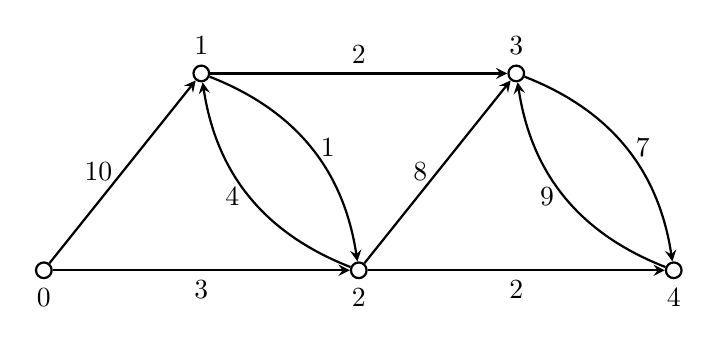
\begin{tikzpicture}
[nodedecorate/.style={shape=circle,inner sep=2pt,draw,thick},%
  arrowdecorate/.style={->,>=stealth,thick}]
% nodes or vertices
\node (0) at (0,0) [nodedecorate] {};
\node [below] at (0.south) {$0$};
\node (2) at (4,0) [nodedecorate] {};
\node [below] at (2.south) {$2$};
\node (4) at (8,0) [nodedecorate] {};
\node [below] at (4.south) {$4$};
\node (1) at (2,2.5) [nodedecorate] {};
\node [above] at (1.north) {$1$};
\node (3) at (6,2.5) [nodedecorate] {};
\node [above] at (3.north) {$3$};
% edges or lines
\path
(0) edge[arrowdecorate] node[left]{$10$} (1)
(0) edge[arrowdecorate] node[below]{$3$} (2)
(1) edge[arrowdecorate,bend left] node[right]{$1$} (2)
(1) edge[arrowdecorate] node[above]{$2$} (3)
(2) edge[arrowdecorate,bend left] node[left]{$4$} (1)
(2) edge[arrowdecorate] node[left]{$8$} (3)
(2) edge[arrowdecorate] node[below]{$2$} (4)
(3) edge[arrowdecorate,bend left] node[right]{$7$} (4)
(4) edge[arrowdecorate,bend left] node[left]{$9$} (3);
\end{tikzpicture}
\caption{Searching a weighted digraph using Dijkstra's algorithm.}
\label{fig:graph_algorithms:Dijkstra_algorithm_digraph}
\end{figure}
%sage: M = matrix([[0,10,3,0,0],[0,0,1,2,0],[0,4,0,8,2],[0,0,0,0,7],[0,0,0,9,0]])
%sage: D = DiGraph(M, format="weighted_adjacency_matrix")
%sage: D.plot(edge_labels=True, graph_border=True).show()

\begin{table}[!htbp]
\centering
\begin{tabular}{|ccccc|} \hline
$v_0$         & $v_1$         & $v_2$         & $v_3$         & $v_4$ \\\hline\hline
\underline{0} & $\infty$      & $\infty$      & $\infty$      & $\infty$ \\
              & 10            & \underline{3} & $\infty$      & $\infty$ \\
              & 7             &               & 11            & \underline{5} \\
              & \underline{7} &               & 11            & \\
              &               &               & \underline{9} & \\\hline
\end{tabular}
\caption{Stepping through Dijkstra's algorithm.}
\label{tab:graph_algorithms:working_through_Dijkstra_algorithm}
\end{table}

\begin{example}
Apply Dijkstra's algorithm to the graph in
Figure~\ref{fig:graph_algorithms:Dijkstra_algorithm_digraph}.
\end{example}

\begin{proof}[Solution]
Dijkstra's algorithm applied to the graph in
Figure~\ref{fig:graph_algorithms:Dijkstra_algorithm_digraph} yields
Table~\ref{tab:graph_algorithms:working_through_Dijkstra_algorithm}. The
steps below explain how this table is created.
%
\begin{enumerate}
\item
Start at $v_0$, let $Q = V$ and $F = \emptyset$. Initialize the labels
$L(v)$ to be $\infty$ for all $v \neq v_0$. This is the first row of
the table. Take the vertex $v_0$ out of the queue.

\item
Consider the set of all adjacent nodes to $v_0$. Replace the labels in
the first row by the weights of the associated edges. Underline the
smallest one and take its vertex (i.e. $v_2$) out of the queue. This
is the second row of the table.

\item
Consider the set of all nodes $w$ which are adjacent to $v_2$. Replace
the labels in the second row by $\min(L(w),\, L(v_2) + wt(v_2, w))$.
Underline the smallest one and take its vertex (i.e. $v_4$) out of the
queue. This is the third row of the table.

\item
Finally, start from $v_4$ and find the path to the remaining vertex
$v_3$ in $Q$. Take the smallest distance from $v_0$ to $v_3$. This is
the last row of the table.
\end{enumerate}
\end{proof}

\begin{exercise}
Dijkstra's algorithm applied to the graph in
Figure~\ref{fig:graph_algorithms:Dijkstra_directed_house_graph}
results in
Table~\ref{tab:graph_algorithms:another_walkthrough_Dijkstra}. Verify
the steps to create this table.
\end{exercise}

\begin{figure}[!htbp]
\centering
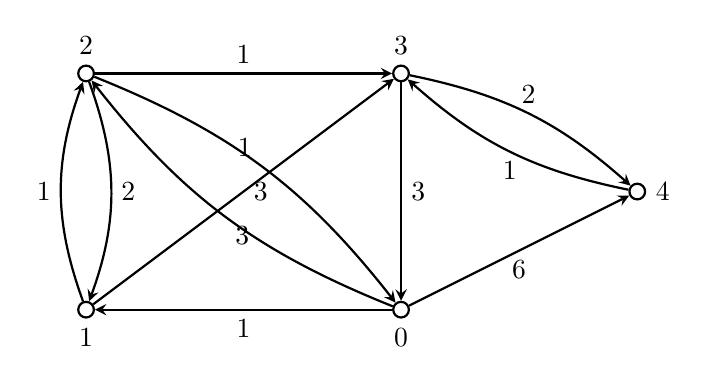
\begin{tikzpicture}
[nodedecorate/.style={shape=circle,inner sep=2pt,draw,thick},%
  arrowdecorate/.style={->,>=stealth,thick}]
% nodes or vertices
\node (0) at (4,0) [nodedecorate] {};
\node [below] at (0.south) {$0$};
\node (1) at (0,0) [nodedecorate] {};
\node [below] at (1.south) {$1$};
\node (2) at (0,3) [nodedecorate] {};
\node [above] at (2.north) {$2$};
\node (3) at (4,3) [nodedecorate] {};
\node [above] at (3.north) {$3$};
\node (4) at (7,1.5) [nodedecorate] {};
\node [right] at (4.east) {$4$};
% edges or lines
\path
(0) edge[arrowdecorate] node[below]{$1$} (1)
(0) edge[arrowdecorate,bend left=15] node[below right]{$3$} (2)
(0) edge[arrowdecorate] node[below]{$6$} (4)
(1) edge[arrowdecorate,bend left=20] node[left]{$1$} (2)
(1) edge[arrowdecorate] node[right]{$3$} (3)
(2) edge[arrowdecorate,bend left=15] node[above left]{$1$} (0)
(2) edge[arrowdecorate,bend left=20] node[right]{$2$} (1)
(2) edge[arrowdecorate] node[above]{$1$} (3)
(3) edge[arrowdecorate] node[right]{$3$} (0)
(3) edge[arrowdecorate,bend left=15] node[above]{$2$} (4)
(4) edge[arrowdecorate,bend left=15] node[below]{$1$} (3);
\end{tikzpicture}
\caption{Searching a directed house graph using Dijkstra's algorithm.}
\label{fig:graph_algorithms:Dijkstra_directed_house_graph}
\end{figure}
%sage: M = matrix([[0,1,3,0,6],[0,0,1,3,0],[1,2,0,1,0],[3,0,0,0,2],[0,0,0,1,0]])
%sage: D = DiGraph(M, format="weighted_adjacency_matrix")
%sage: D.plot(edge_labels=True, graph_border=True).show()

\begin{table}[!htbp]
\centering
\begin{tabular}{|ccccc|} \hline
$v_0$         & $v_1$         & $v_2$         & $v_3$         & $v_4$ \\\hline\hline
\underline{0} & $\infty$      & $\infty$      & $\infty$      & $\infty$ \\
              & \underline{1} & 3             & $\infty$      & 6 \\
              &               & \underline{2} & 4             & 6 \\
              &               &               & \underline{3} & 6 \\
              &               &               &               & \underline{5} \\\hline
\end{tabular}
\caption{Another walk-through of Dijkstra's algorithm.}
\label{tab:graph_algorithms:another_walkthrough_Dijkstra}
\end{table}


%%-----------------------------------------------------------------------%%
%%--- Bellman-Ford algorithm --------------------------------------------%%

\subsection{Bellman-Ford algorithm}

See section~24.1 of Cormen~et~al.~\cite{CormenEtAl2001}, and
section~8.5 of Berman and Paul~\cite{BermanPaul1997}.

The Bellman-Ford algorithm computes single-source shortest paths in a
weighted graph or digraph, where some of the edge weights may be
negative. Instead of the ``greedy'' approach that Dijkstra's algorithm
took, i.e. searching for the ``cheapest'' path, the Bellman-Ford
algorithm searches over all edges and keeps track of the shortest one
found as it searches.

The implementation below takes in a graph or digraph, and creates two
Python dictionaries \verb!dist! and \verb!predecessor!, keyed on the
list of vertices, which store the distance and shortest
paths. However, if a negative weight cycle exists~(in the case of a
digraph), then an error is raised.

\begin{center}
\fontsize{9pt}{9pt}
\selectfont
\tt
\begin{lstlisting}
def bellman_ford(Gamma, s):
    """
    Computes the shortest distance from s to all other vertices in Gamma.
    If Gamma has a negative weight cycle, then return an error.

    INPUT:

    - Gamma -- a graph.
    - s -- the source vertex.

    OUTPUT:

    - (d,p) -- pair of dictionaries keyed on the list of vertices,
      which store the distance and shortest paths.

    REFERENCE:

    http://en.wikipedia.org/wiki/Bellman-Ford_algorithm
    """
    P = []
    dist = {}
    predecessor = {}
    V = Gamma.vertices()
    E = Gamma.edges()
    for v in V:
        if v == s:
            dist[v] = 0
        else:
            dist[v] = infinity
        predecessor[v] = 0
    for i in range(1, len(V)):
        for e in E:
            u = e[0]
            v = e[1]
            wt = e[2]
            if dist[u] + wt < dist[v]:
                dist[v] = dist[u] + wt
                predecessor[v] = u
    # check for negative-weight cycles
    for e in E:
        u = e[0]
        v = e[1]
        wt = e[2]
        if dist[u] + wt < dist[v]:
            raise ValueError("Graph contains a negative-weight cycle")
    return dist, predecessor
\end{lstlisting}
\end{center}

Bellman-Ford runs in $O(|V|\cdot |E|)$-time, which is $O(n^3)$ for
``dense'' connected graphs (where $n=|V|$).

Here are some examples.

\begin{center}
\fontsize{9pt}{9pt}
\selectfont
\tt
\begin{lstlisting}
sage: M = matrix([[0,1,4,0], [0,0,1,5], [0,0,0,3], [0,0,0,0]])
sage: G = Graph(M, format="weighted_adjacency_matrix")
sage: bellman_ford(G, G.vertices()[0])
  {0: 0, 1: 1, 2: 2, 3: 5}
\end{lstlisting}
\end{center}
%
The plot of this graph is given in
Figure~\ref{fig:graph_algorithms:Bellman_Ford_example}.

\begin{figure}[!htbp]
\centering
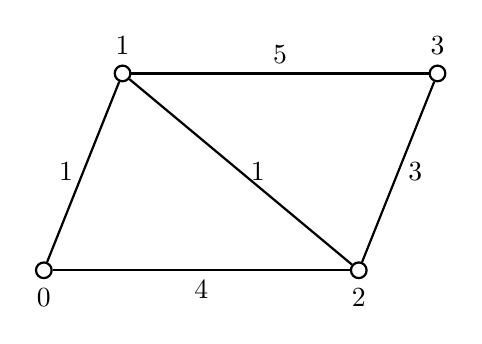
\begin{tikzpicture}
[nodedecorate/.style={shape=circle,inner sep=2pt,draw,thick},%
  linedecorate/.style={-,thick}]
% nodes or vertices
\node (0) at (0,0) [nodedecorate] {};
\node [below] at (0.south) {$0$};
\node (2) at (4,0) [nodedecorate] {};
\node [below] at (2.south) {$2$};
\node (1) at (1,2.5) [nodedecorate] {};
\node [above] at (1.north) {$1$};
\node (3) at (5,2.5) [nodedecorate] {};
\node [above] at (3.north) {$3$};
% edges or lines
\path
(0) edge[linedecorate] node[left]{$1$} (1)
(0) edge[linedecorate] node[below]{$4$} (2)
(1) edge[linedecorate] node[right]{$1$} (2)
(1) edge[linedecorate] node[above]{$5$} (3)
(2) edge[linedecorate] node[right]{$3$} (3);
\end{tikzpicture}
\caption{Shortest paths in a weighted graph using the Bellman-Ford
  algorithm.}
\label{fig:graph_algorithms:Bellman_Ford_example}
\end{figure}
%sage: M = matrix([[0,1,4,0],[0,0,1,5],[0,0,0,3],[0,0,0,0]])
%sage: G = Graph(M, format = "weighted_adjacency_matrix")
%sage: G.plot(graph_border=True, edge_labels=True).show()

The following example illustrates the case of a negative-weight cycle.

\begin{center}
\fontsize{9pt}{9pt}
\selectfont
\tt
\begin{lstlisting}
sage: M = matrix([[0,1,0,0],[1,0,-4,1],[1,1,0,0],[0,0,1,0]])
sage: G = DiGraph(M, format = "weighted_adjacency_matrix")
sage: bellman_ford(G, G.vertices()[0])
---------------------------------------------------------------------------
...
ValueError: Graph contains a negative-weight cycle
\end{lstlisting}
\end{center}
%
The plot of this graph is given in
Figure~\ref{fig:graph_algorithms:Bellman_Ford_negative_weights}.

\begin{figure}[!htbp]
\centering
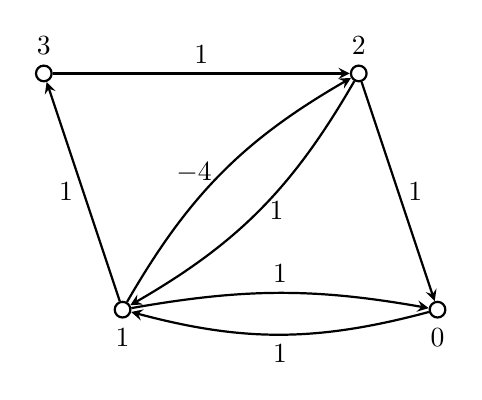
\begin{tikzpicture}
[nodedecorate/.style={shape=circle,inner sep=2pt,draw,thick},%
  arrowdecorate/.style={->,>=stealth,thick}]
% nodes or vertices
\node (0) at (5,0) [nodedecorate] {};
\node [below] at (0.south) {$0$};
\node (1) at (1,0) [nodedecorate] {};
\node [below] at (1.south) {$1$};
\node (2) at (4,3) [nodedecorate] {};
\node [above] at (2.north) {$2$};
\node (3) at (0,3) [nodedecorate] {};
\node [above] at (3.north) {$3$};
% edges or lines
\path
(0) edge[arrowdecorate,bend left=15] node[below]{$1$} (1)
(1) edge[arrowdecorate,bend left=10] node[above]{$1$} (0)
(1) edge[arrowdecorate,bend left=15] node[left]{$-4$} (2)
(1) edge[arrowdecorate] node[left]{$1$} (3)
(2) edge[arrowdecorate] node[right]{$1$} (0)
(2) edge[arrowdecorate,bend left=15] node[right]{$1$} (1)
(3) edge[arrowdecorate] node[above]{$1$} (2);
\end{tikzpicture}
\caption{Searching a digraph with negative weight using the
  Bellman-Ford algorithm.}
\label{fig:graph_algorithms:Bellman_Ford_negative_weights}
\end{figure}
%sage: M = matrix([[0,1,0,0],[1,0,-4,1],[1,1,0,0],[0,0,1,0]])
%sage: G = Graph(M, format = "weighted_adjacency_matrix")
%sage: G.plot(graph_border=True, edge_labels=True).show()


%%-----------------------------------------------------------------------%%
%%--- Floyd-Warshall algorithm ------------------------------------------%%

\subsection{Floyd-Roy-Warshall algorithm}

See section~25.2 of Cormen~et~al.~\cite{CormenEtAl2001}, and section
14.4 of Berman and Paul~\cite{BermanPaul1997}.

The \emph{Floyd-Roy-Warshall algorithm}~(FRW), or the Floyd-Warshall
algorithm, is an algorithm for finding shortest paths in a weighted,
directed graph. Like the Bellman-Ford algorithm, it allows for
negative edge weights and detects a negative weight cycle if one
exists. Assuming that there are no negative weight cycles, a single
execution of the FRW algorithm will find the shortest paths between
all pairs of vertices. It was discovered independently by Bernard Roy
in 1959, Robert Floyd in 1962, and by Stephen Warshall in 1962.

In some sense, the FRW algorithm is an example of
``dynamic programming,'' which allows one to break the computation
into simpler steps using some sort of recursive procedure. The rough
idea is as follows. Temporarily label the vertices of $G$ as
$V = \{1,2,\dots,n\}$. Call $SD(i,j,k)$ a shortest distance from
vertex $i$ to vertex $j$ that only uses vertices $1$ through $k$. This
can be computed using the recursive expression
\[
SD(i,j,k)
=
\min\{ SD(i,j,k-1),\, SD(i,k,k-1) + SD(k,j,k-1)\}.
\]
The key to the Floyd-Roy-Warshall algorithm lies in exploiting this
formula. If $n = |V|$, then this is a $O(n^3)$ time algorithm. For
comparison, the Bellman-Ford algorithm has complexity
$O(|V| \cdot |E|)$, which is $O(n^3)$ time for ``dense''
graphs. However, Bellman-Ford only yields the shortest paths emanating
from a \emph{single} vertex. To achieve comparable output, we would
need to iterate Bellman-Ford over \emph{all} vertices, which would be
an  $O(n^4)$ time algorithm for ``dense'' graphs. Except possibly for
``sparse'' graphs, Floyd-Roy-Warshall is better than an iterated
implementation of Bellman-Ford.

Here is an implementation in Sage.
%
\begin{center}
\fontsize{9pt}{9pt}
\selectfont
\tt
\begin{lstlisting}
def floyd_roy_warshall(A):
    """
    Shortest paths

    INPUT:

    - A -- weighted adjacency matrix

    OUTPUT:

    - dist -- a matrix of distances of shortest paths.
    - paths -- a matrix of shortest paths.
    """
    G = Graph(A, format="weighted_adjacency_matrix")
    V = G.vertices()
    E = [(e[0],e[1]) for e in G.edges()]
    n = len(V)
    dist = [[0]*n for i in range(n)]
    paths = [[-1]*n for i in range(n)]
    # initialization step
    for i in range(n):
        for j in range(n):
            if (i,j) in E:
                paths[i][j] = j
            if i == j:
                dist[i][j] = 0
            elif A[i][j]<>0:
                dist[i][j] = A[i][j]
            else:
                dist[i][j] = infinity
    # iteratively finding the shortest path
    for j in range(n):
        for i in range(n):
            if i <> j:
                for k in range(n):
                    if k <> j:
                        if dist[i][k]>dist[i][j]+dist[j][k]:
                            paths[i][k] = V[j]
                        dist[i][k] = min(dist[i][k], dist[i][j] +dist[j][k])
    for i in range(n):
        if dist[i][i] < 0:
            raise ValueError, "A negative edge weight cycle exists."
    return dist, matrix(paths)
\end{lstlisting}
\end{center}

Here are some examples.

%
%\begin{center}
%\fontsize{9pt}{9pt}
%\selectfont
%\tt
%\begin{lstlisting}
%
%        sage: A = matrix([[0,1,2,3],[0,0,2,1],[20,10,0,3],[11,12,13,0]]); A
%        sage: floyd_roy_warshall(A)
%        ([[0, 1, 2, 2], [12, 0, 2, 1], [14, 10, 0, 3], [11, 12, 13, 0]],
%          [-1  1  2  1]
%          [ 3 -1  2  3]
%          [ 3 -1 -1  3]
%          [-1 -1 -1 -1])
%
%\end{lstlisting}
%\end{center}
%

%
%\begin{center}
%\fontsize{9pt}{9pt}
%\selectfont
%\tt
%\begin{lstlisting}
%
%        sage: A = matrix([[0,1,2,4],[0,0,2,1],[0,0,0,5],[0,0,0,0]])
%        sage: floyd_roy_warshall(A)
%        ([[0, 1, 2, 2], [+Infinity, 0, 2, 1], [+Infinity, +Infinity, 0, 5],
%          [+Infinity, +Infinity, +Infinity, 0]],
%          [-1  1  2  1]
%          [-1 -1  2  3]
%          [-1 -1 -1  3]
%          [-1 -1 -1 -1])
%
%\end{lstlisting}
%\end{center}
%

\begin{center}
\fontsize{9pt}{9pt}
\selectfont
\tt
\begin{lstlisting}
sage: A = matrix([[0,1,2,3],[0,0,2,1],[-5,0,0,3],[1,0,1,0]]); A
sage: floyd_roy_warshall(A)
Traceback (click to the left of this block for traceback)
...
ValueError: A negative edge weight cycle exists.
\end{lstlisting}
\end{center}

The plot of this weighted digraph with four vertices appears in
Figure~\ref{fig:graph_algorithms:Floyd_Roy_Warshall_demo}.

\begin{figure}[!htbp]
\centering
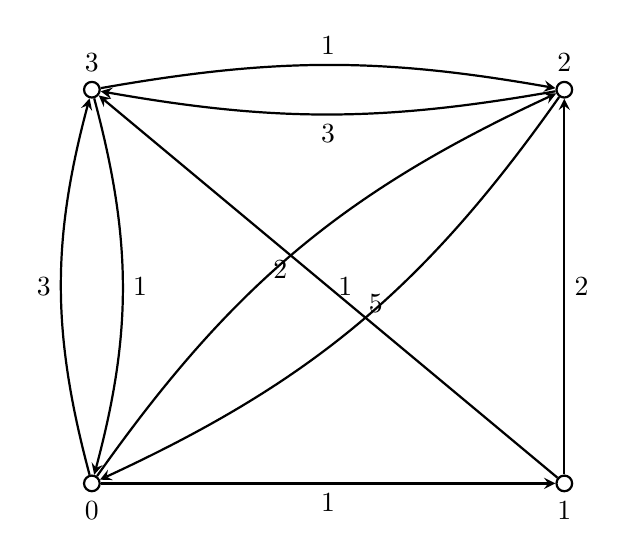
\begin{tikzpicture}
[nodedecorate/.style={shape=circle,inner sep=2pt,draw,thick},%
  arrowdecorate/.style={->,>=stealth,thick}]
% nodes or vertices
\node (0) at (0,0) [nodedecorate] {};
\node [below] at (0.south) {$0$};
\node (1) at (6,0) [nodedecorate] {};
\node [below] at (1.south) {$1$};
\node (2) at (6,5) [nodedecorate] {};
\node [above] at (2.north) {$2$};
\node (3) at (0,5) [nodedecorate] {};
\node [above] at (3.north) {$3$};
% edges or lines
\path
(0) edge[arrowdecorate] node[below]{$1$} (1)
(0) edge[arrowdecorate,bend left=15] node[below left]{$2$} (2)
(0) edge[arrowdecorate,bend left=15] node[left]{$3$} (3)
(1) edge[arrowdecorate] node[right]{$2$} (2)
(1) edge[arrowdecorate] node[right]{$1$} (3)
(2) edge[arrowdecorate,bend left=15] node[above right]{$5$} (0)
(2) edge[arrowdecorate,bend left=10] node[below]{$3$} (3)
(3) edge[arrowdecorate,bend left=15] node[right]{$1$} (0)
(3) edge[arrowdecorate,bend left=10] node[above]{$1$} (2);
\end{tikzpicture}
\caption{Demonstrating the Floyd-Roy-Warshall algorithm.}
\label{fig:graph_algorithms:Floyd_Roy_Warshall_demo}
\end{figure}
%sage: A = matrix([[0,1,2,3],[0,0,2,1],[-5,0,0,3],[1,0,1,0]])
%sage: D = DiGraph(A, format="weighted_adjacency_matrix")
%sage: D.plot(edge_labels=True, graph_border=True).show()

\begin{center}
\fontsize{9pt}{9pt}
\selectfont
\tt
\begin{lstlisting}
sage: A = matrix([[0,1,2,3],[0,0,2,1],[-1/2,0,0,3],[1,0,1,0]]); A
sage: floyd_roy_warshall(A)
([[0, 1, 2, 2], [3/2, 0, 2, 1], [-1/2, 1/2, 0, 3/2], [1/2, 3/2, 1, 0]],
  [-1  1  2  1]
  [ 2 -1  2  3]
  [-1  0 -1  1]
  [ 2  2 -1 -1])
\end{lstlisting}
\end{center}

The plot of this weighted digraph with four vertices appears in
Figure~\ref{fig:graph_algorithms:another_Floyd_Roy_Warshall_demo}.

\begin{figure}[!htbp]
\centering
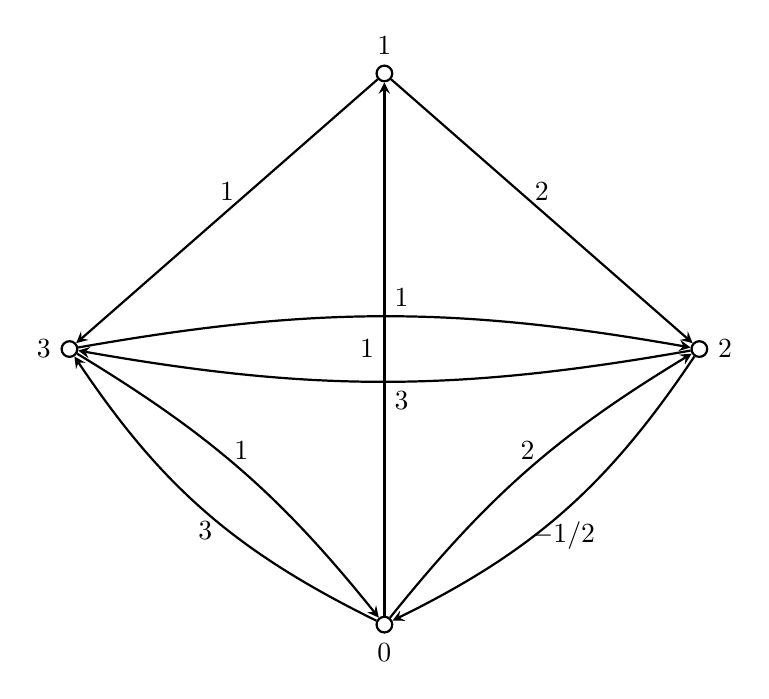
\begin{tikzpicture}
[nodedecorate/.style={shape=circle,inner sep=2pt,draw,thick},%
  arrowdecorate/.style={->,>=stealth,thick}]
% nodes or vertices
\node (0) at (0,0) [nodedecorate] {};
\node [below] at (0.south) {$0$};
\node (1) at (0,7) [nodedecorate] {};
\node [above] at (1.north) {$1$};
\node (2) at (4,3.5) [nodedecorate] {};
\node [right] at (2.east) {$2$};
\node (3) at (-4,3.5) [nodedecorate] {};
\node [left] at (3.west) {$3$};
% edges or lines
\path
(0) edge[arrowdecorate] node[left]{$1$} (1)
(0) edge[arrowdecorate,bend left=10] node[above]{$2$} (2)
(0) edge[arrowdecorate,bend left=15] node[below]{$3$} (3)
(1) edge[arrowdecorate] node[above]{$2$} (2)
(1) edge[arrowdecorate] node[above]{$1$} (3)
(2) edge[arrowdecorate,bend left=15] node[below]{$-1/2$} (0)
(2) edge[arrowdecorate,bend left=10] node[below right]{$3$} (3)
(3) edge[arrowdecorate,bend left=10] node[above]{$1$} (0)
(3) edge[arrowdecorate,bend left=10] node[above right]{$1$} (2);
\end{tikzpicture}
\caption{Another demonstration of the Floyd-Roy-Warshall algorithm.}
\label{fig:graph_algorithms:another_Floyd_Roy_Warshall_demo}
\end{figure}
%sage: A = matrix([[0,1,2,3],[0,0,2,1],[-1/2,0,0,3],[1,0,1,0]])
%sage: D = DiGraph(A, format="weighted_adjacency_matrix")
%sage: D.plot(edge_labels=True, graph_border=True).show()



%%-----------------------------------------------------------------------%%
%%--- Johnson's algorithm -----------------------------------------------%%

\subsection{Johnson's algorithm}

See section~25.3 of Cormen~et~al.~\cite{CormenEtAl2001} and
Johnson~\cite{Johnson1977}.

Let $G = (V,E)$ be a graph with edge weights but no negative cycles.
\emph{Johnson's algorithm} finds a shortest path between all pairs of
vertices in a ``sparse'' directed graph.
\index{Johnson's algorithm}

%\begin{itemize}
%\item
%Add a new vertex $v_0$ with zero weight edges from it to all $v\in V$.
%
%\item
%Run the Bellman-Ford algorithm to check for negative weight cycles
%and find $h(v)$,
%the least weight of a path from the new node $v_0$ to $v\in V$.
%If this step detects a negative cycle, the algorithm is terminated.
%
%\item
%Reweight the edges using the vertices' $h(v)$ values: an edge from
%$v\in V$ to $w\in V$, having length $wt(v,w)$, is given the new length
%$wt(v,w) + h(v) - h(w)$.
%
%\item
%For each $v\in V$, run Dijkstra's algorithm and store the computed
%least weight to other vertices.
%\end{itemize}

\begin{algorithm}[!htpb]
\dontprintsemicolon  % no semicolon at end of pseudocode statements
%% data section
\SetKwInOut{Input}{Input}
\SetKwInOut{Output}{Output}
\SetKwData{Count}{count}
\SetKwData{False}{False}
\SetKwData{True}{True}
%% input/output
\Input{A connected graph $G = (V, E)$ having (possibly negative) edge
  weights.}
\Output{A shortest path between all pairs of vertices in $V$
  (or terminate if a negative edge cycle is detected).}
\BlankLine
%% algorithm body
Add a new vertex $v_0$ with zero weight edges from it to all $v \in V$.\;

Run the Bellman-Ford algorithm to check for negative weight cycles
and find $h(v)$, the least weight of a path from the new node $v_0$ to
$v \in V$.

If the last step detects a negative cycle, the algorithm is terminated.\;

Re-weight the edges using the vertices' $h(v)$ values: an edge from
$v \in V$ to $w \in V$, having length $wt(v,w)$, is given the new length
$wt(v,w) + h(v) - h(w)$.\;

For each $v \in V$, run Dijkstra's algorithm and store the computed
least weight to other vertices.
\caption{Johnson's algorithm.}
\label{alg:graph_algorithms:johnson}
\end{algorithm}

The time complexity, for sparse graphs, is
$O(|V|^2\log |V| + |V| \cdot |E)|=O(n^2\log n)$, where $n = |V|$ is
the number of vertices of the original graph $G$.
